\section{Dataset (\textsc{Qur’an-MD})}
\label{sec:dataset-preparation}

The dataset was constructed by aggregating and harmonizing three publicly available sources of Qur’anic data: (1) a Kaggle dataset of verse-level speech-to-text recordings by 30 reciters \cite{quran_ayat_speech_kaggle}, (2) the \texttt{quranwbw} repository containing aligned word-by-word Arabic text, English translations, and transliterations \cite{quranwbw_repo}, and (3) the Internet Archive collection of word-by-word Qur’an audio recordings \cite{quran_wordbyword_archive}. To unify these heterogeneous resources, we designed a hierarchical JSON template. At the top level, each \texttt{surah} (chapter) is represented by its numerical index (e.g., \texttt{"112"} for the 114 surah's) and annotated with its Arabic name, English translation, transliteration, and total verse count. Each surah contains a nested set of \texttt{verses} (ayahs), where each verse entry includes the Arabic text, its English translation, phonetic transliteration, paths to reciter-specific verse-level audio, and a list of word-level objects. Word objects store the word Arabic script, English translation, transliteration, and the corresponding aligned audio file. This structure allows seamless integration of textual, transliterated, and auditory modalities across both verse- and word-level granularities.  

The preparation pipeline proceeded in four main steps. First, surah-level metadata (surah number, names, and verse counts) was populated into the template. Second, from the Kaggle dataset, verse-level recitations by 30 reciters were aligned with their corresponding verse texts and added under the \texttt{audio\_ayah\_path} field. Third, word-level Arabic text, translations, and transliterations from the \texttt{quranwbw} repository were inserted into the template. Fourth, word-level audio files from the Internet Archive collection were matched to individual tokens and linked under the \texttt{audio\_word\_path} field. After populating all layers, automated validation scripts were applied to ensure correctness, checking that every word and verse was paired with its corresponding audio, and identifying and correcting missing or misaligned entries. This pipeline resulted in a complete, consistent, and multimodal representation of the Qur’an, ready for release as a standardized dataset.

\textbf{Dataset Format}: The dataset is organized in a hierarchical JSON structure, where each surah (chapter) of the Qur’an is represented as a nested object. This design ensures that verse-level and word-level information is consistently accessible and easily parsable for downstream applications. An example of Surah 112 (\textit{Al-Ikhlas}) is shown in Figure \ref{fig:example} (Appendix), highlighting metadata and audio/text linkage. This structure enables researchers to work seamlessly at both the verse level (for example, analyzing prosody between reciters) and the word level (for example, studying phoneme-grapheme alignment).

\begin{figure}[htp]
    \centering
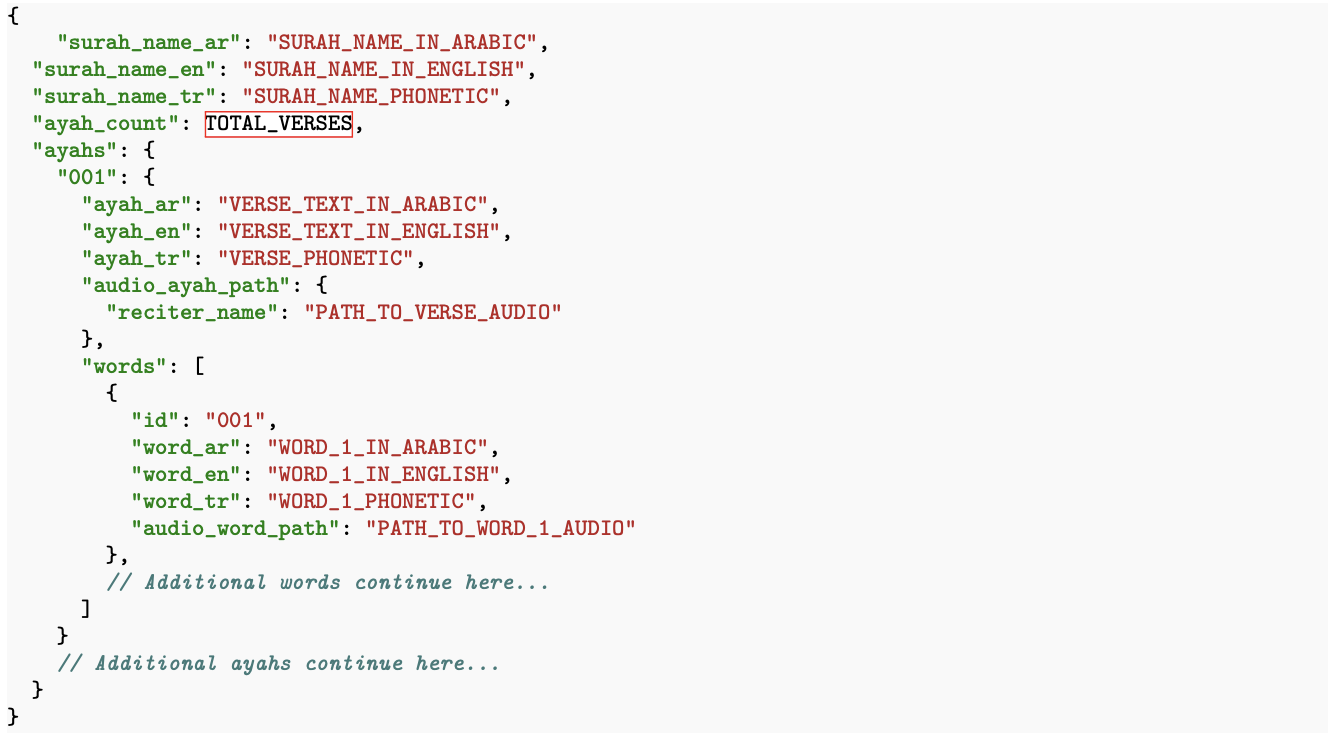
\includegraphics[width=\textwidth]{figures/fing.png} % Adjust width as needed
    % \caption{Example of format of Surah 112 (Al-Ikhlas) in the Dataset.}
    \label{fig:fing}
\end{figure}

% \begin{minted}[fontsize=\scriptsize, breaklines, bgcolor=lightgray!10]{json}
% { 
%     "surah_name_ar": "SURAH_NAME_IN_ARABIC",
%   "surah_name_en": "SURAH_NAME_IN_ENGLISH",
%   "surah_name_tr": "SURAH_NAME_PHONETIC",
%   "ayah_count": TOTAL_VERSES,
%   "ayahs": {
%     "001": {
%       "ayah_ar": "VERSE_TEXT_IN_ARABIC",
%       "ayah_en": "VERSE_TEXT_IN_ENGLISH",
%       "ayah_tr": "VERSE_PHONETIC",
%       "audio_ayah_path": {
%         "reciter_name": "PATH_TO_VERSE_AUDIO"
%       },
%       "words": [
%         {
%           "id": "001",
%           "word_ar": "WORD_1_IN_ARABIC",
%           "word_en": "WORD_1_IN_ENGLISH",
%           "word_tr": "WORD_1_PHONETIC",
%           "audio_word_path": "PATH_TO_WORD_1_AUDIO"
%         },
%         // Additional words continue here...
%       ]
%     }
%     // Additional ayahs continue here...
%   }
% }
% \end{minted}